%!TEX root = ./main.tex

\section[Distance]{Ruler 2: Compare Two Frequencies (Chronos)}

% SECTION TIMING: 42:00--62:00 (6 frames). Chronos's story in its own pictures. The
% symmetry IS the pedagogy: same trick as the last section with "position" and
% "frequency" swapped. Say "a difference across a small step beats wrapping" in both
% sections, in the same words.

% Teaching note (120 s): the constraint that motivates everything: homes and shops
% have ONE access point. One AP can give a bearing; to pin a point it also needs the
% distance. And distance = speed of light x propagation delay, which lives in the
% phase -- wrapped, as we saw.
\begin{frame}{Homes have ONE access point}
  \vspace{0.2em}
  \centering
  
\includegraphics[width=0.7\textwidth]{figure/ch_one_ap.png}

  \vspace{0.5em}
  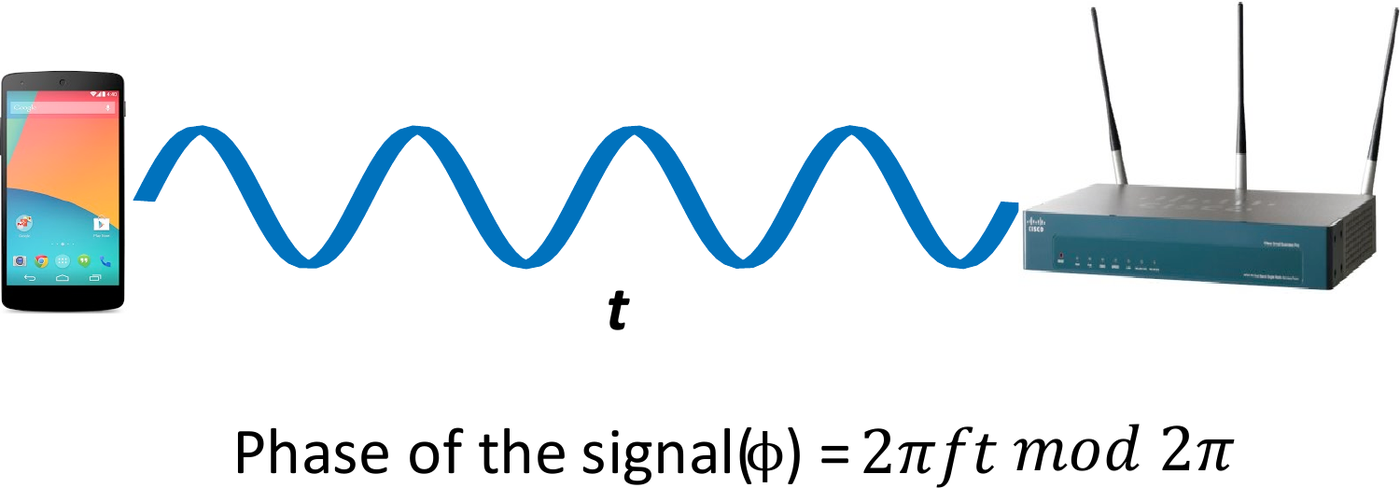
\includegraphics[width=0.6\textwidth]{figure/ch_prop_delay.png}

  \vspace{0.3em}
  {\small One AP needs angle \emph{and} distance. Distance $= c \times$ propagation
   delay, and the delay sits in the phase --- wrapped.\par}
  \source{https://www.usenix.org/conference/nsdi16/technical-sessions/presentation/vasisht}{Figures: Chronos talk, NSDI 2016}
\end{frame}

% Teaching note (210 s): THE intuition frame of the section. One frequency: the ticks
% repeat every period, so the delay is ambiguous. Add a second frequency: it repeats
% at a different period. Only at the TRUE delay do the ticks of every frequency line
% up (the green check). Mathematicians call it the Chinese remainder theorem; the
% class can call it "find the time when all four clocks agree".
\begin{frame}{Many frequencies agree on only one delay}
  \vspace{0.2em}
  \centering
  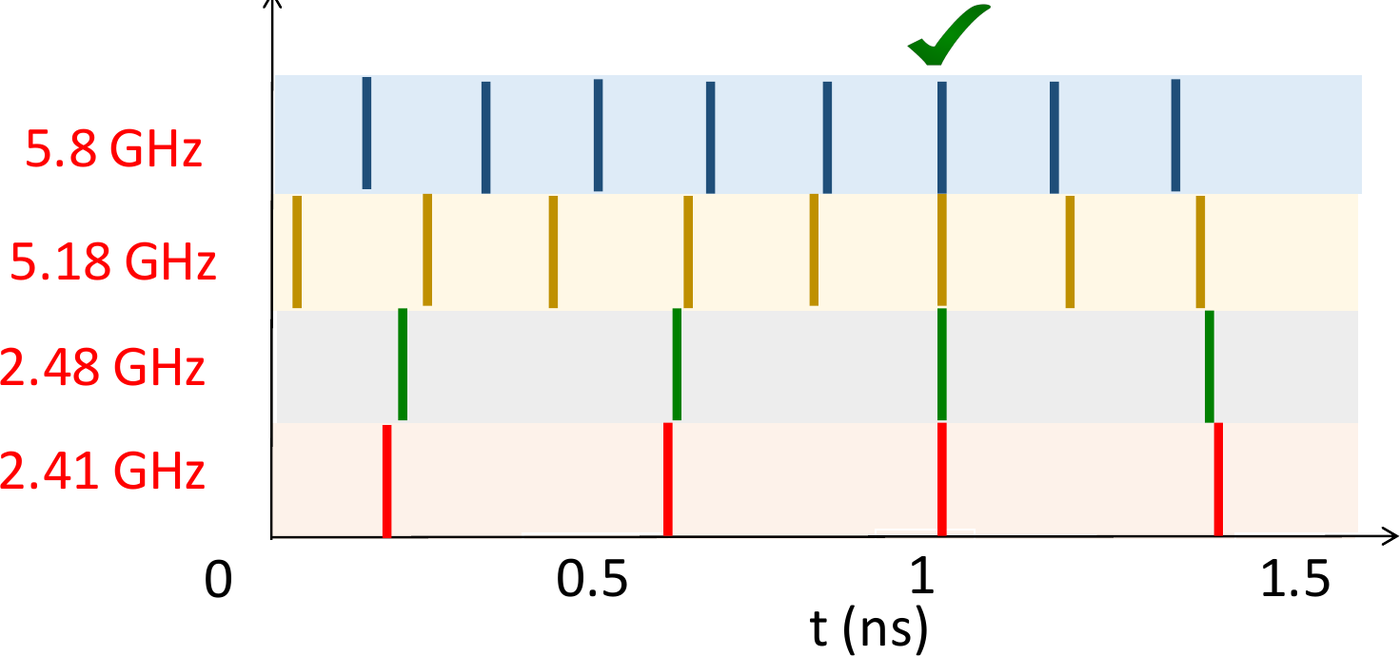
\includegraphics[width=0.7\textwidth]{figure/ch_many_freqs.png}

  \vspace{0.4em}
  {\small Each frequency wraps at its own period. Only the true delay is consistent
   with \emph{all} of them.\par}
  \vspace{0.3em}
  \takeaway{Same sentence as last section: a \textbf{difference across a small
    step} beats wrapping --- now the step is in frequency, not space.}
  \source{https://www.usenix.org/conference/nsdi16/technical-sessions/presentation/vasisht}{Figure: Chronos talk, NSDI 2016}
\end{frame}

% Teaching note (180 s): where do many frequencies come from, measured at the same
% instant? OFDM -- Class 8. A Wi-Fi packet is 52+ subcarriers delta apart, each with
% its own phase. Plot phase against subcarrier: a straight line whose slope is the
% delay. For a 5 m path the line falls ~120 degrees across a 20 MHz packet.
\begin{frame}{OFDM hands you the frequencies for free}
  \vspace{0.2em}
  \centering
  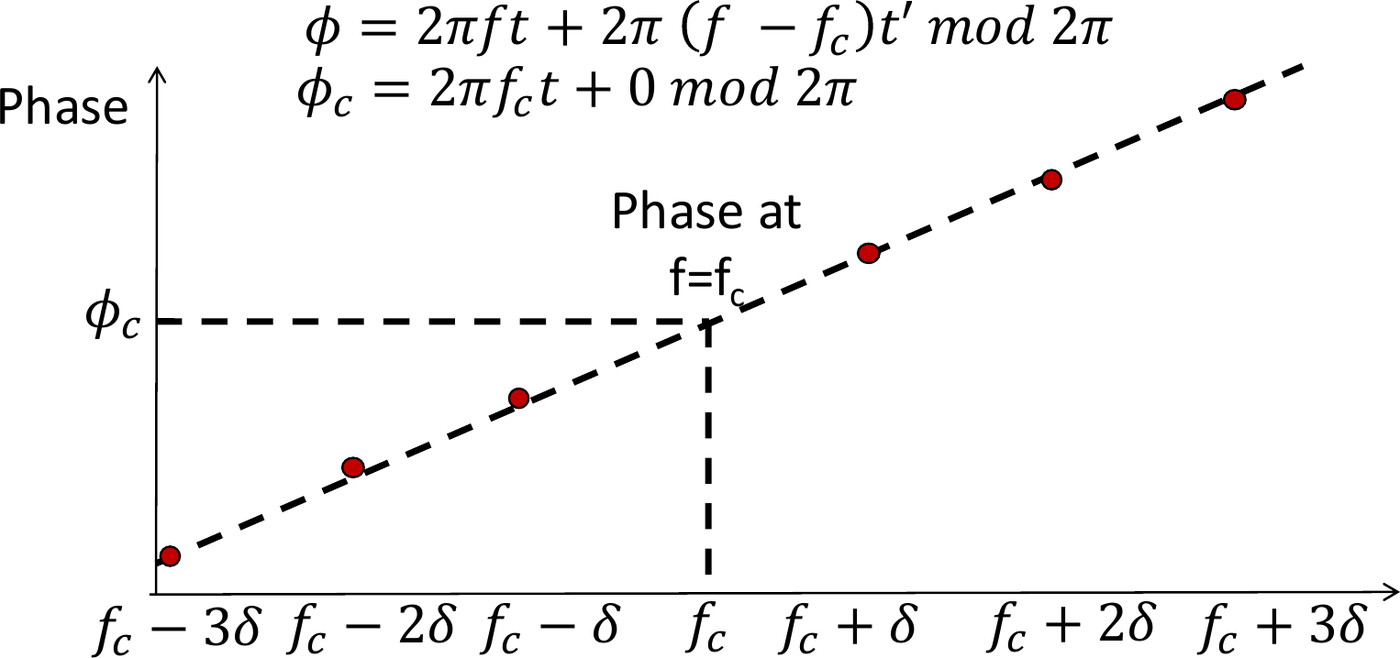
\includegraphics[width=0.74\textwidth]{figure/ch_ofdm_slope.png}

  \vspace{0.3em}
  {\small Phase vs.\ subcarrier is a \textbf{straight line}; its slope is the
   delay. 5 m path: $\approx 120^\circ$ of fall across one 20 MHz packet.\par}
  \vspace{0.3em}
  \takeaway{You have known this since Class 8: every packet is 52+ equally spaced
    tones, each reporting its own phase.}
  \source{https://www.usenix.org/conference/nsdi16/technical-sessions/presentation/vasisht}{Figure: Chronos talk, NSDI 2016}
\end{frame}

% Teaching note (180 s): multipath, resolved honestly. Each path has its own delay;
% transform the phase-vs-frequency line back to time (IFFT across subcarriers) and
% you get the channel impulse response -- one spike per path. Reflections travel
% farther by definition, so the SHORTEST delay is the distance to the phone.
\begin{frame}{Multipath: the shortest delay is the distance}
  \vspace{0.2em}
  \begin{columns}[T,onlytextwidth]
    \column{0.5\textwidth}
      \centering
      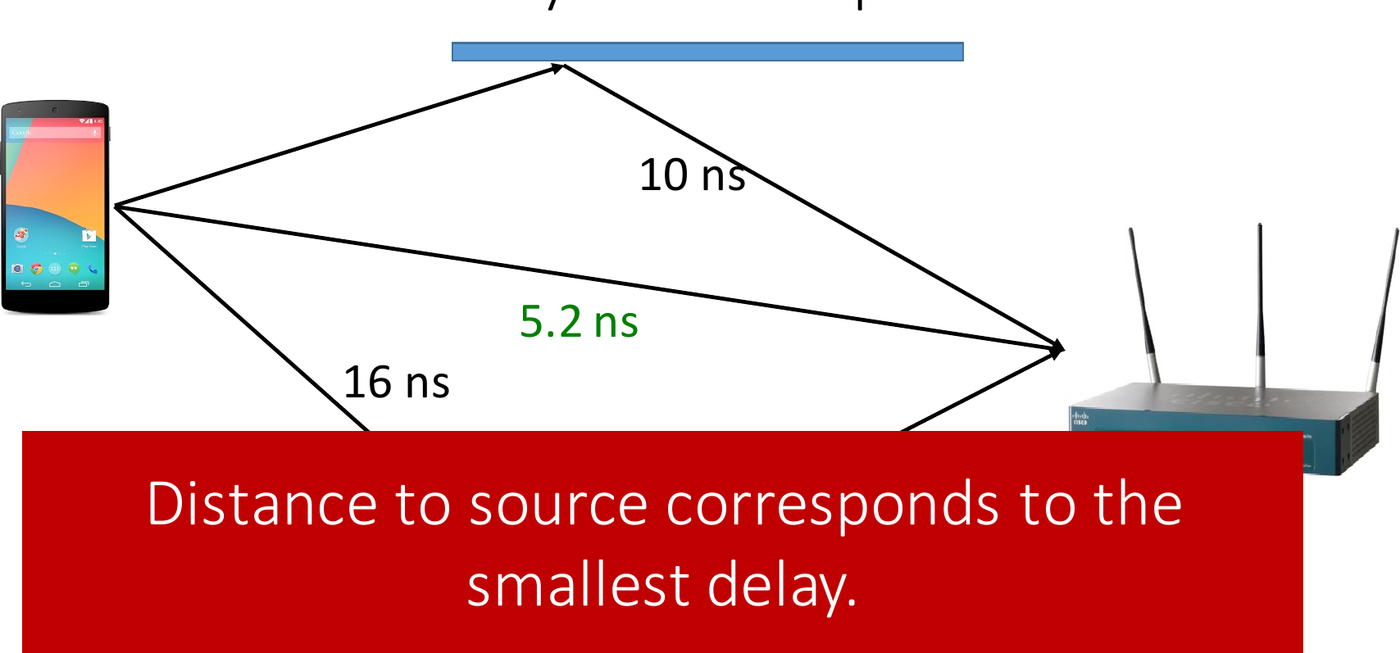
\includegraphics[width=\linewidth]{figure/ch_smallest_delay.png}
    \column{0.47\textwidth}
      \centering
      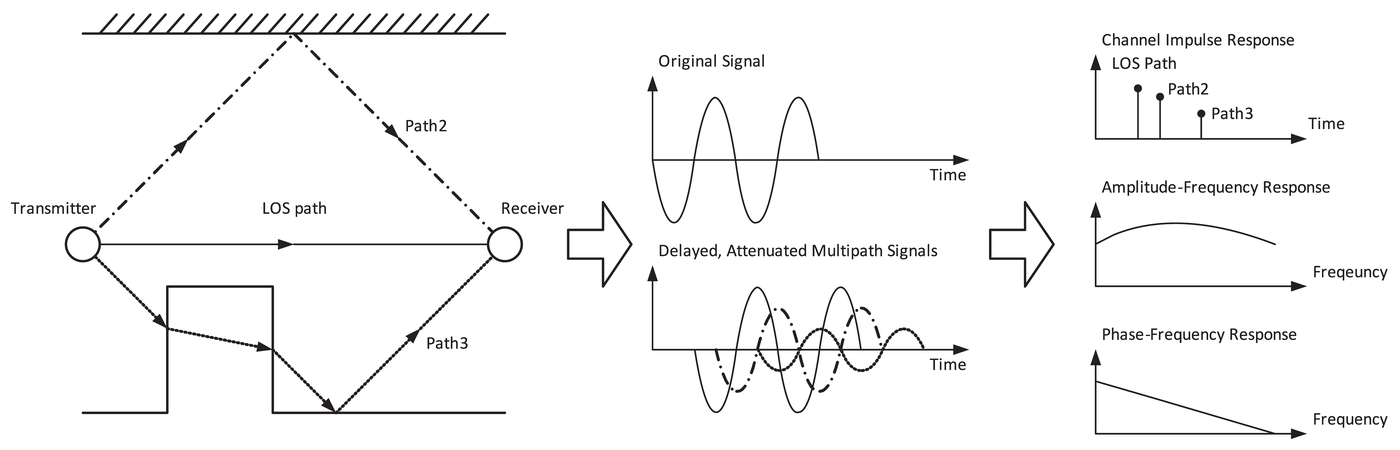
\includegraphics[width=\linewidth]{figure/tsinghua_multipath_cir.png}
      {\small IFFT across subcarriers: one spike per path.\par}
  \end{columns}
  \vspace{0.4em}
  {\small A reflection always travels farther. 5.2 ns $\times$ $c$ $=$ 1.6 m to
   the phone.\par}
  \source{https://tns.thss.tsinghua.edu.cn/wst/docs/pre/}{Figures: Chronos talk, NSDI 2016 (left); Yang et al., Tsinghua ``Hands-on Wireless Sensing'' tutorial (right)}
\end{frame}

% Teaching note (210 s): the honesty frame. The AP cannot see the propagation delay
% alone: it sees propagation + its own packet-DETECTION delay, which is larger and
% differs on every packet. Chronos's two moves: the phase at the carrier frequency
% is immune to detection delay (read it off the OFDM line), and a packet/ACK exchange
% cancels the unknown clock offset. Also the resolution limit: a 20 MHz packet
% separates delays only ~15 m apart, so Chronos hops across every Wi-Fi band.
\begin{frame}{The catch: the receiver's own delay}
  \vspace{0.2em}
  \centering
  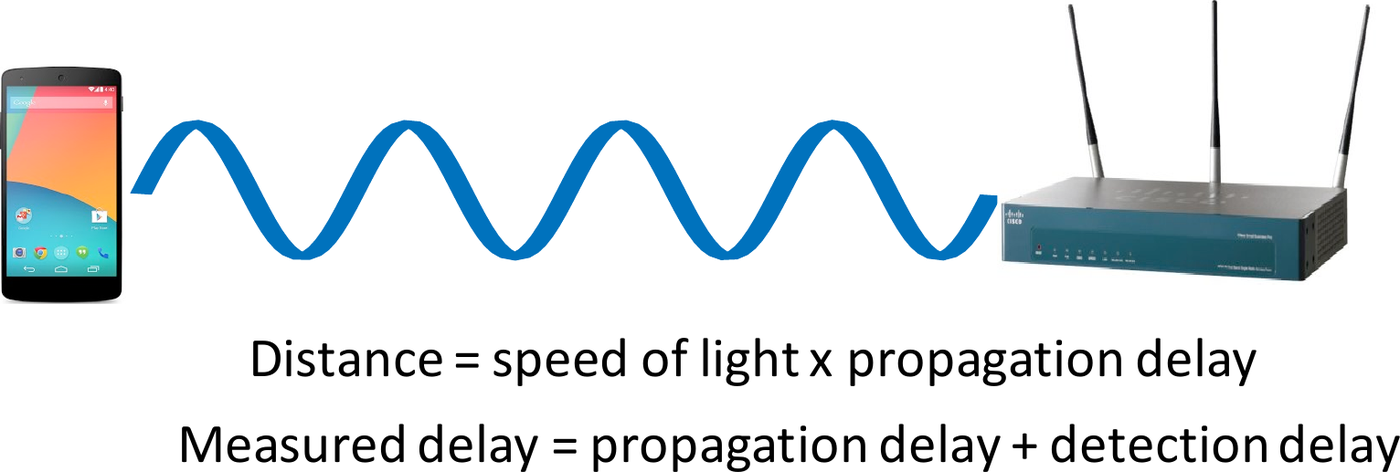
\includegraphics[width=0.84\textwidth]{figure/ch_detection_delay.png}

  \vspace{0.3em}
  \raggedright
  {\small
   \begin{itemize}\itemsep2pt
     \item Detection delay is larger than propagation delay and changes every packet.
     \item Chronos: the phase \emph{at the carrier} is immune --- read it off the
       OFDM line; a packet/ACK pair cancels clock offsets.
     \item Resolution is bandwidth: 20 MHz separates paths only $\sim$15 m apart,
       so Chronos hops across all Wi-Fi bands.
   \end{itemize}\par}
  \source{https://www.usenix.org/conference/nsdi16/technical-sessions/presentation/vasisht}{Figure: Chronos talk, NSDI 2016}
\end{frame}

% Teaching note (120 s): what one stock AP buys you: 14 cm distance error with line
% of sight, the right room 94% of the time, a drone that keeps 1.4 m from its user
% to within 4 cm. Say the hardware out loud: an Intel 5300 Wi-Fi card.
\begin{frame}{What a single access point achieves}
  \vspace{0.2em}
  \begin{columns}[T,onlytextwidth]
    \column{0.31\textwidth}
      \centering
      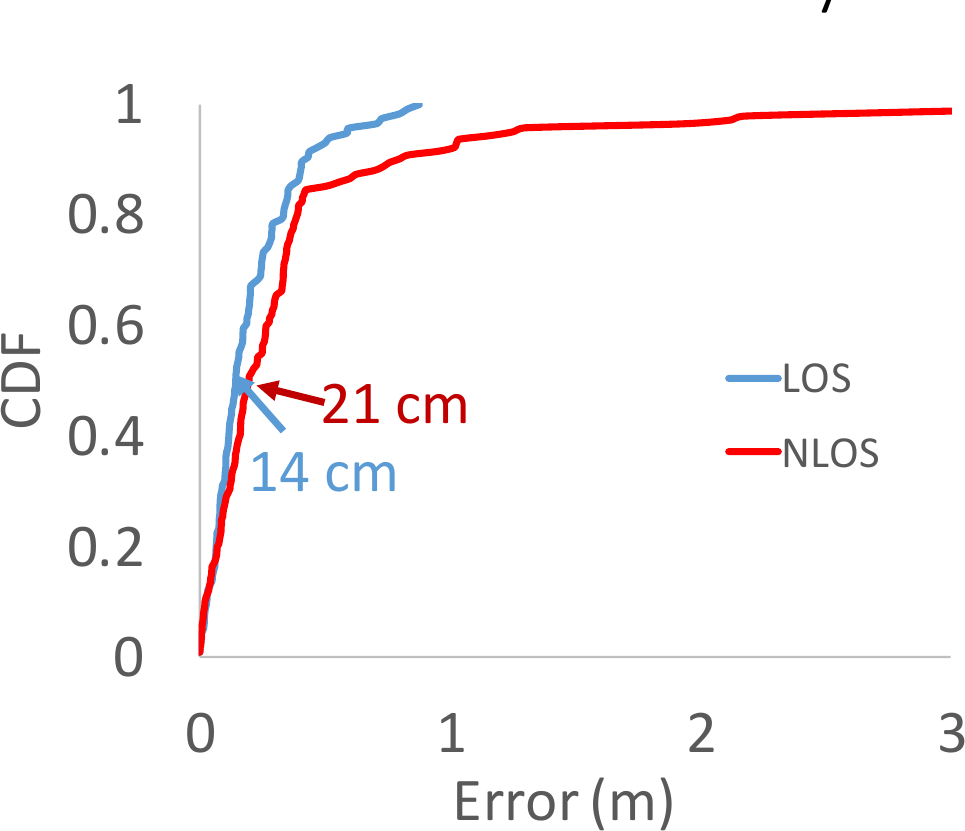
\includegraphics[width=\linewidth]{figure/ch_distance_cdf.png}
      {\small Distance: \textbf{14 cm} (LOS), 21 cm (NLOS)\par}
    \column{0.33\textwidth}
      \centering
      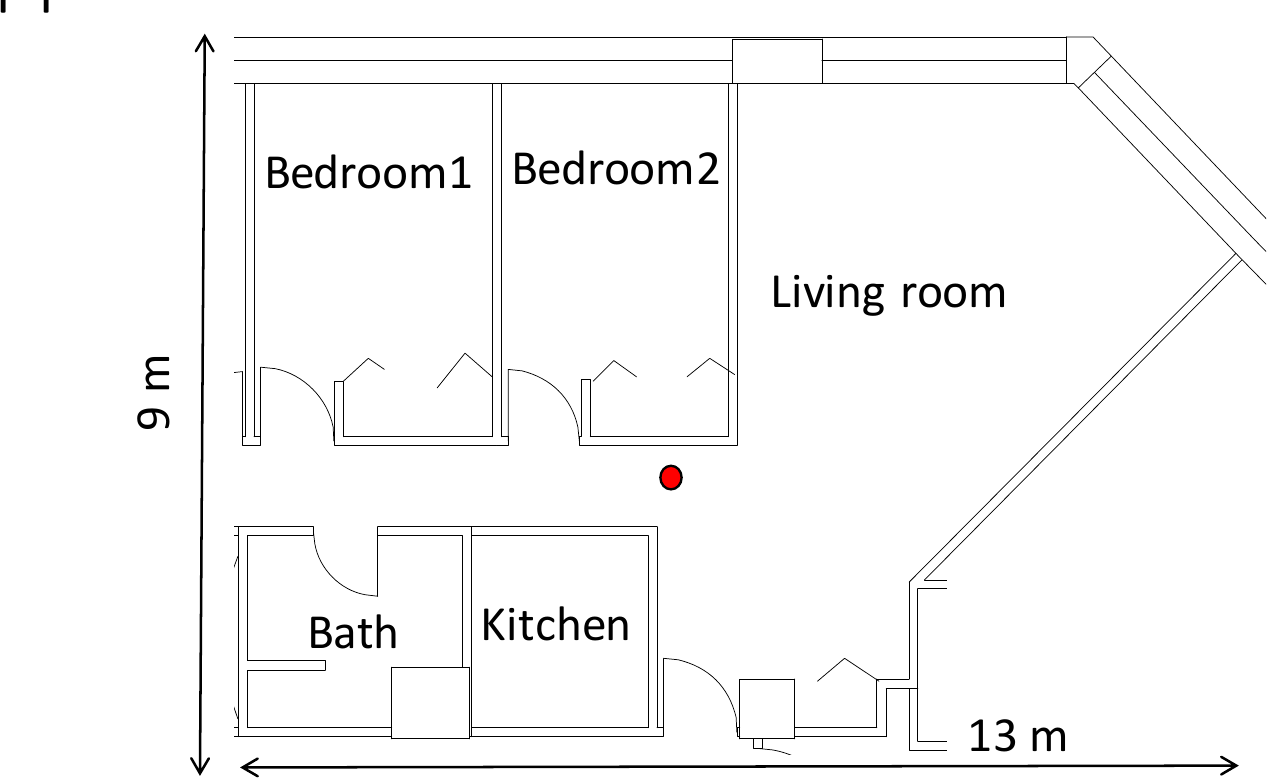
\includegraphics[width=\linewidth]{figure/ch_smart_home.png}
      {\small Right room \textbf{94\%} of the time\par}
    \column{0.31\textwidth}
      \centering
      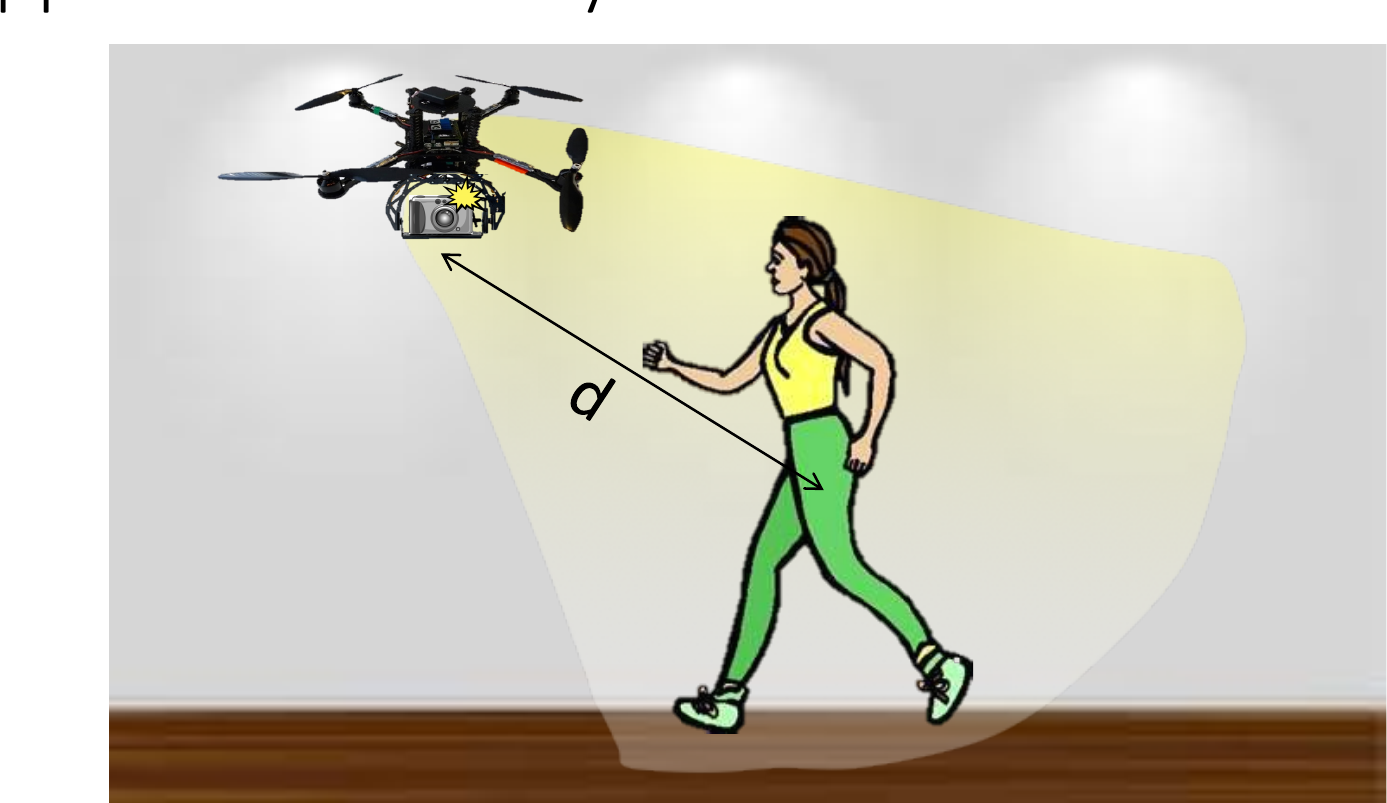
\includegraphics[width=\linewidth]{figure/ch_drone.png}
      {\small Drone follows at 1.4 m, \textbf{4 cm} error\par}
  \end{columns}
  \vspace{0.5em}
  \takeaway{One off-the-shelf Wi-Fi card. No infrastructure beyond the AP.}
  \source{https://www.usenix.org/conference/nsdi16/technical-sessions/presentation/vasisht}{Figures: Chronos talk, NSDI 2016}
\end{frame}
